\iffalse
\let\negmedspace\undefined
\let\negthickspace\undefined
\documentclass[journal,12pt,twocolumn]{IEEEtran}
\usepackage{cite}
\usepackage{amsmath,amssymb,amsfonts,amsthm}
\usepackage{algorithmic}
\usepackage{graphicx}
\usepackage{textcomp}
\usepackage{xcolor}
\usepackage{txfonts}
\usepackage{listings}
\usepackage{enumitem}
\usepackage{mathtools}
\usepackage{gensymb}
\usepackage{comment}
\usepackage[breaklinks=true]{hyperref}
\usepackage{tkz-euclide} 
\usepackage{listings}
\usepackage{gvv}                                        
\def\inputGnumericTable{}                                 
\usepackage[latin1]{inputenc}                                
\usepackage{color}                                            
\usepackage{array}                                            
\usepackage{longtable}                                       
\usepackage{calc}                                             
\usepackage{multirow}                                         
\usepackage{hhline}                                           
\usepackage{ifthen}                                           
\usepackage{lscape}
\newtheorem{theorem}{Theorem}[section]
\newtheorem{problem}{Problem}
\newtheorem{proposition}{Proposition}[section]
\newtheorem{lemma}{Lemma}[section]
\newtheorem{corollary}[theorem]{Corollary}
\newtheorem{example}{Example}[section]
\newtheorem{definition}[problem]{Definition}
\newcommand{\BEQA}{\begin{eqnarray}}
\newcommand{\EEQA}{\end{eqnarray}}
\newcommand{\define}{\stackrel{\triangle}{=}}
\theoremstyle{remark}
\newtheorem{rem}{Remark}
\begin{document}

\bibliographystyle{IEEEtran}
\vspace{3cm}

\title{GATE: CH - 60.2022}
\author{EE23BTECH11224 - Sri Krishna Prabhas Yadla$^{*}$% <-this % stops a space
}
\maketitle
\newpage
\bigskip

\renewcommand{\thefigure}{\arabic{figure}}
\renewcommand{\thetable}{\arabic{table}}


\vspace{3cm}
\textbf{Question:} Consider a single-input-single-output (SISO) system with the transfer function
\begin{align*}
G_p(s) = \frac{2\brak{s+1}}{\brak{\frac{1}{2}s+1}\brak{\frac{1}{4}s+1}}
\end{align*}
where the time constants are in minutes. The system is forced by a unit step input at
time $t = 0$. The time at which the output response reaches the maximum is \rule{1cm}{0.15mm} minutes (rounded off to two decimal places). \hfill (GATE CH 2022)\\
\solution
\fi
\begin{table}[htbp]
	\centering
	\def\arraystretch{1.5}
	\begin{tabular}{|c|c|c|}
\hline
\textbf{Parameters} & \textbf{Description} & \textbf{Value} \\
\hline
$y(t)$ & Output response & \\
\hline
$G_p(s)$ & Transfer function & $\frac{2\brak{s+1}}{\brak{\frac{1}{2}s+1}\brak{\frac{1}{4}s+1}}$\\
\hline
$x(t)$ & Input & $u(t)$ \\
\hline
	$X(s)$ & Laplace transform of x(t) & $\frac{1}{s}$\\
\hline
$y'(t)$ & $\frac{dy}{dt}$ &  \\
\hline
\end{tabular}

	\caption{Parameters}
	\label{tab:parameters_ch_60}
\end{table}
\begin{align}
Y(s) &= G_p(s)X(s) \\
&= \frac{16\brak{s+1}}{s\brak{s+2}\brak{s+4}}\\
&= \frac{2}{s}+\frac{4}{s+2}-\frac{6}{s+4} \\
\label{ch60_L(u)} u(t) &\system{L} \frac{1}{s} \\
\label{ch60_L(e^-at)} e^{-at} u(t) &\system{L} \frac{1}{s+a}
\end{align}
From Laplace transforms \eqref{ch60_L(u)} and \eqref{ch60_L(e^-at)}, we get
\begin{align}
y(t) &= \brak{2+4e^{-2t}-6e^{-4t}}u(t)
\end{align}
For maximum value of $y(t)$,
\begin{align}
y'(t) &= 0\\
\implies -8e^{-2t}+24e^{-4t} &= 0\\
e^{2t} &= 3\\
\implies t &= \frac{\ln{3}}{2} \\
&\approx 0.55
\end{align}
\begin{figure}[htbp]
	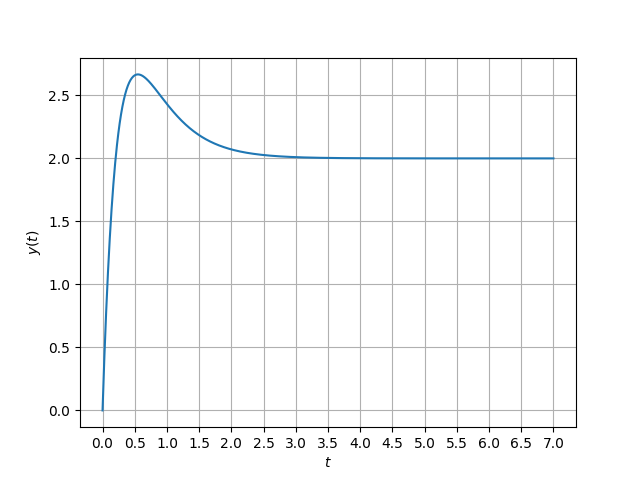
\includegraphics[width=\columnwidth]{2022/CH/60/figs/plot.png}
	\caption{Plot of $y(t)$}
	\label{fig:plot_ch60}
\end{figure}
